In this exercise, we will write two small computer programs for random
walks on a $2D$ square lattice:
\begin{itemize}
    \item one for the usual random walk, where the walker is allowed to 
        come back to points already visited
    \item one for the so-called self-avoiding random walk (SAW), 
        where the walker is not allowed to do so and hence does not 
        cross its own path.
\end{itemize}
HINT: One can find a lot of algorithms for the SAW in the web. It is ok 
to use just the simplest one: When the walker revisits a position, you 
discard the walk. Otherwise you use the trajectory. Note that this 
algorithm for the SAW is not very efficient (you have to reject more 
and more trajectories for larger $n$), so you should restrict yourself 
to $n<N$ with, say, $N=30$. For the usual random walk there is no such 
problem and you can explore larger $N$.

\paragraph{a) Write the program for a typical RW} \ \\
\\

\paragraph{b) Write the program for a SAW} \ \\
\\

\paragraph{c) Show some representative trajectories.} \ \\
\\
    \begin{figure}[h!]
        \centering
        \begin{minipage}{.5\linewidth}
          \centering
          \subfloat[normal random walk ($n=400$)]{
            \label{:a}
            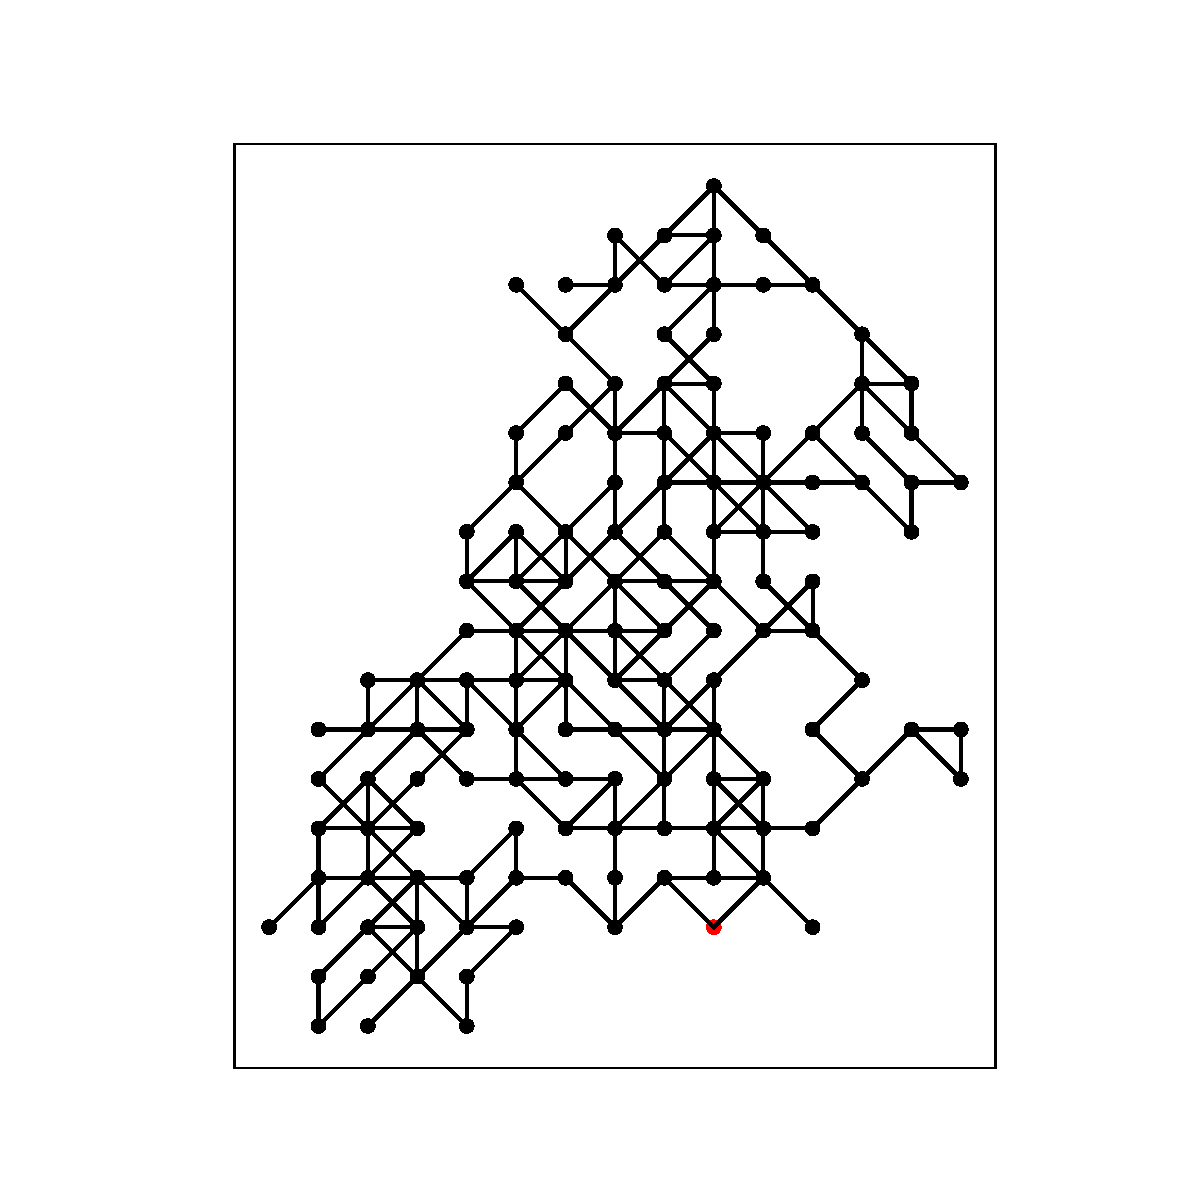
\includegraphics[scale=.5]{./figures/RW_good.pdf}
          }
        \end{minipage}%
        \begin{minipage}{.5\linewidth}
          \centering
          \subfloat[self-avoiding random walk $n=30$]{
            \label{:b}
            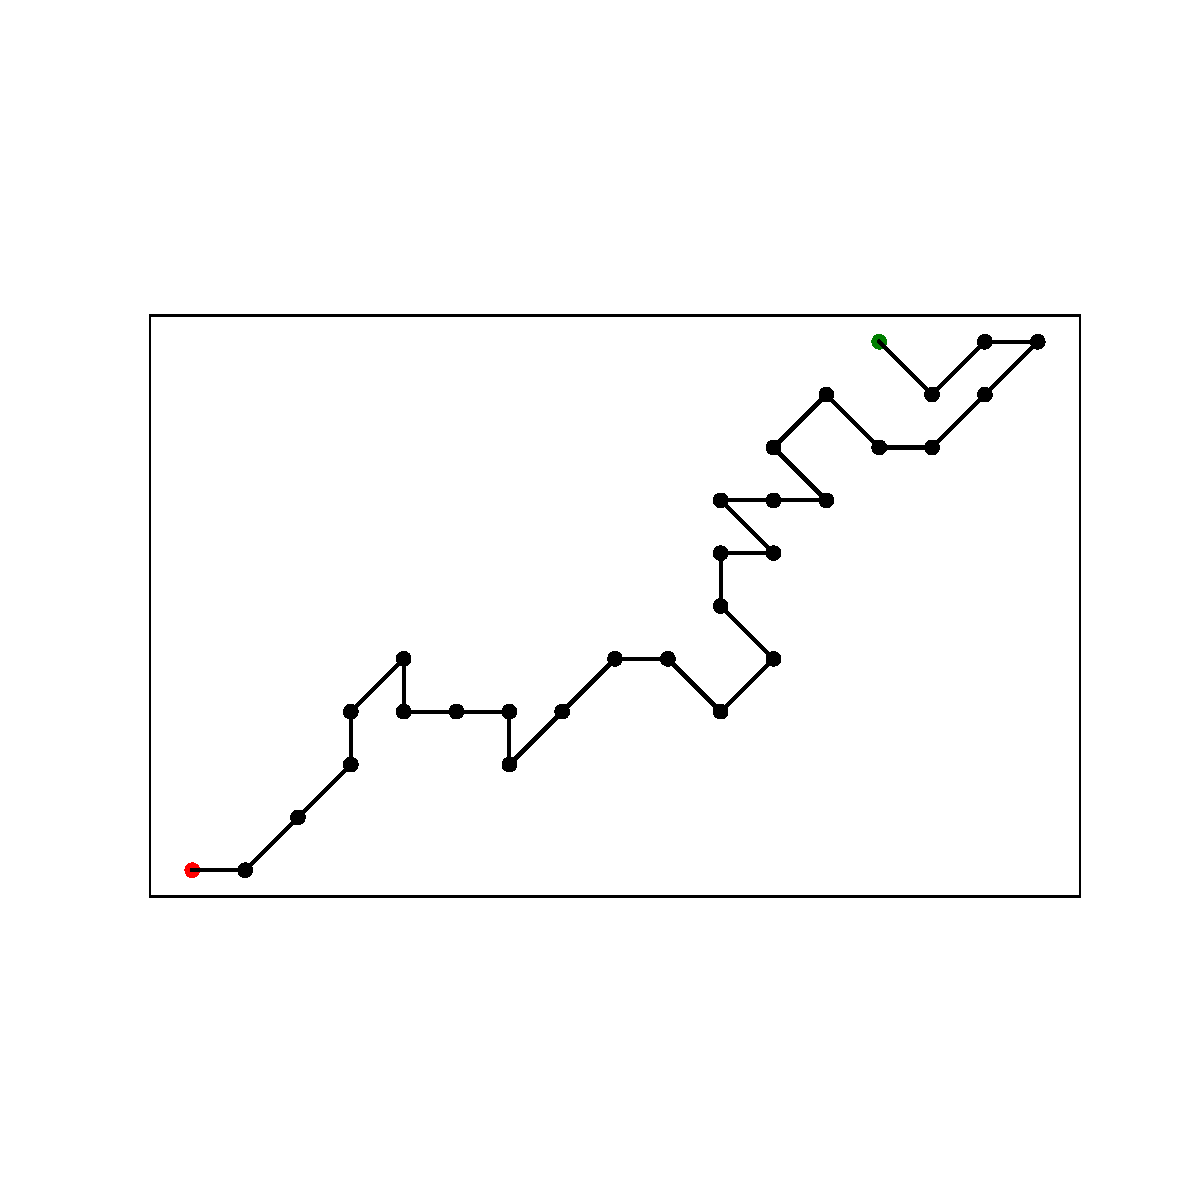
\includegraphics[scale=.5]{./figures/SAW_good.pdf}
          }
        \end{minipage}
    \end{figure} \ \\

\paragraph{d) Measure the mean squared displacements (MSD) 
    $\langle x^2(n)\rangle$ as a function of the number of steps $n$ 
    for both cases (the average is over different trajectories). If you 
    plot the results in log-log-scale you can extract the exponents 
    $\alpha$, where $\langle x^2(n)\rangle\sim n\alpha$, for the two 
    cases. Compare and discuss.
} \ \\
\\
    \begin{figure}[h!]
        \centering
        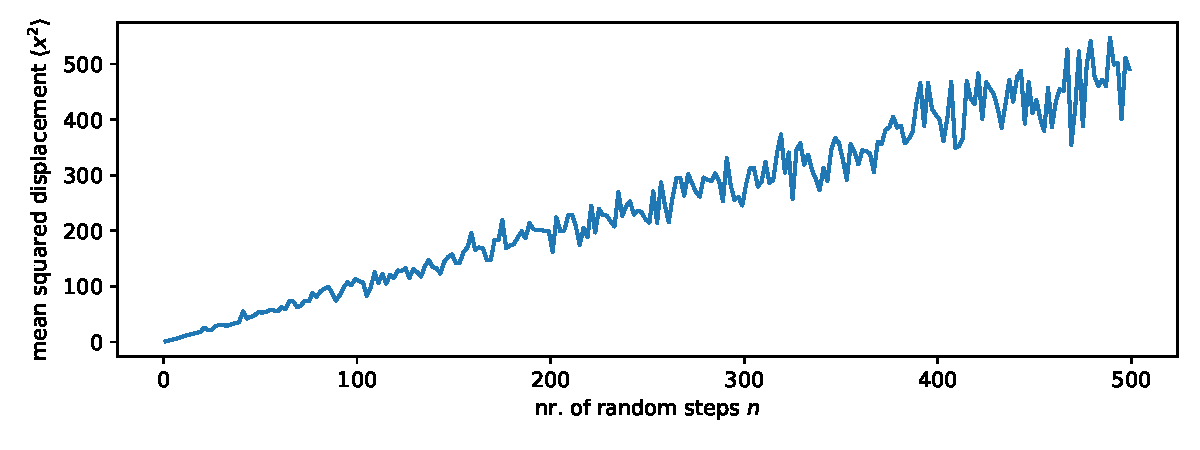
\includegraphics[width=\textwidth]{./figures/MSD_vs_N.pdf}
        \caption{}
    \end{figure} \ \\ 

